\section{Results}

\begin{landscape}\label{data}
\begin{longtable}[]{@{}lllcccc@{}}
	\caption{Time ranges, mean age per bin, corresponding stratigraphic stages and epochs, and respective sample sizes (on individual, species and genus level).)}
	\label{tab:bins}\tabularnewline
	\toprule
	Age Range [mya] & Mean Age [mya] & Stages & Epochs & n (Individuals) & n (Species) & n (Genera)\tabularnewline
	\midrule
	\endhead
	0 - 0.0117 & 0.00585 & Modern & Modern & 254 & 66 & 18\tabularnewline
	0.0117 - 0.126 & 0.06885 & Upper Pleistocene & Upper Pleistocene & 50
	& 18 & 8\tabularnewline
	0.126 - 0.781 & 0.45350 & Middle Pleistocene & Middle Pleistocene & 53
	& 13 & 7\tabularnewline
	0.781 - 1.81 & 1.29350 & Lower Pleistocene & Lower Pleistocene & 57 &
	27 & 12\tabularnewline
	1.81 - 2.59 & 2.19700 & Gelasian & Lower Pleistocene & 33 & 15 &
	9\tabularnewline
	2.59 - 3.6 & 3.09400 & Piacencian & Upper Pliocene & 24 & 15 &
	10\tabularnewline
	3.6 - 5.33 & 4.46600 & Zanclean & Lower Pliocene & 31 & 17 &
	8\tabularnewline
	5.33 - 7.25 & 6.28900 & Messinian & Upper Miocene & 12 & 9 &
	6\tabularnewline
	7.25 - 11.6 & 9.42700 & Tortonian & Upper Miocene & 46 & 20 &
	9\tabularnewline
	11.6 - 13.8 & 12.71400 & Serravallian & Middle Miocene & 27 & 8 &
	6\tabularnewline
	13.8 - 16 & 14.89500 & Langhian & Middle Miocene & 18 & 14 &
	9\tabularnewline
	16 - 23 & 19.50000 & Burdigalian/Aquitanian & Lower Miocene & 31 & 15 & 9\tabularnewline
	\bottomrule
\end{longtable}
\end{landscape}



%__________________________________________________________________
\begin{figure}[htbp]
	\centering
	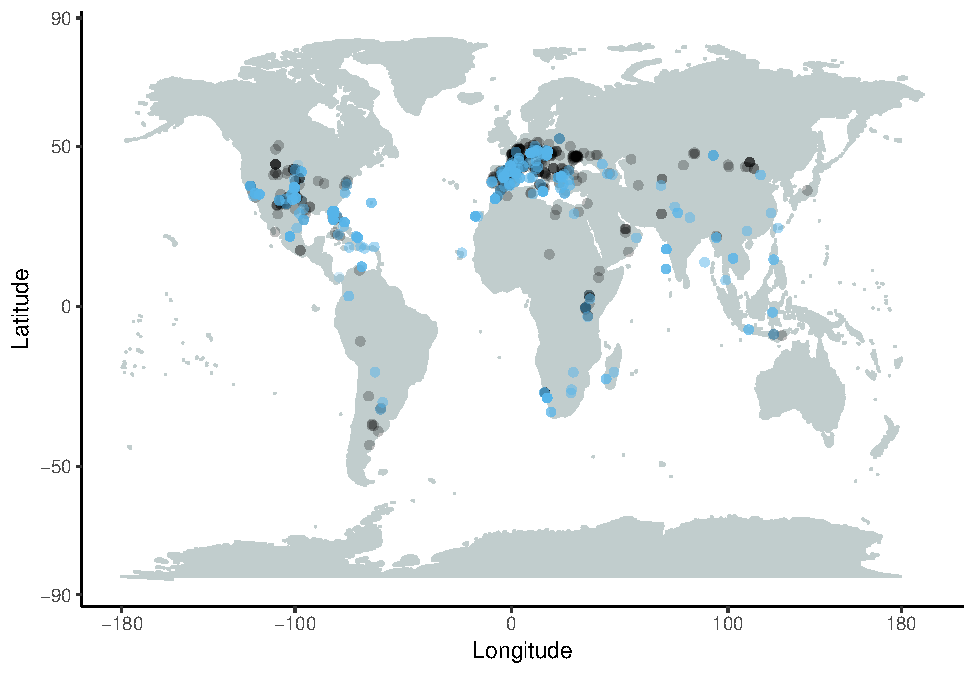
\includegraphics{MA_JJ_files/figure-latex/MapFossilOccurrences-1.pdf}
	\caption{Map displaying all fossil occurrences of testudinids, with
		color indicating whether body size data was available (blue) or not (black).}
\end{figure}




%______________________________________________________________________
\begin{figure}[htbp]
	\centering
	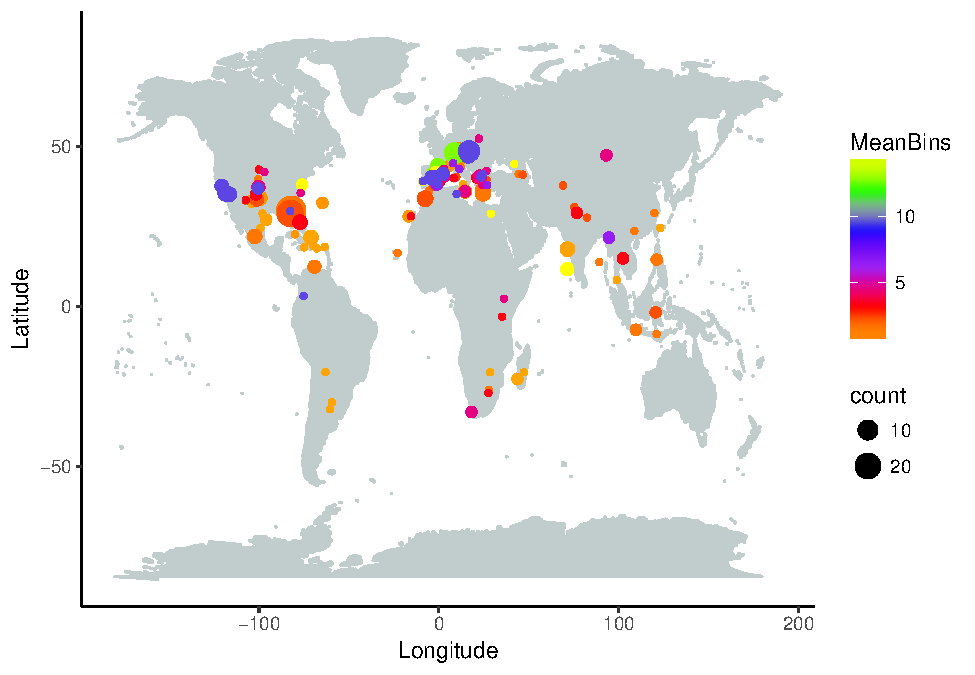
\includegraphics{MA_JJ_files/figure-latex/MapCL-1.pdf}
	\caption{Map displaying all localities for which body size data for
		testudinids was available in the literature. Size of points denotes
		sample size, color denotes approximate age.}
\end{figure}




%_______________________________________________________________________
\begin{figure}[htbp]
	\centering
	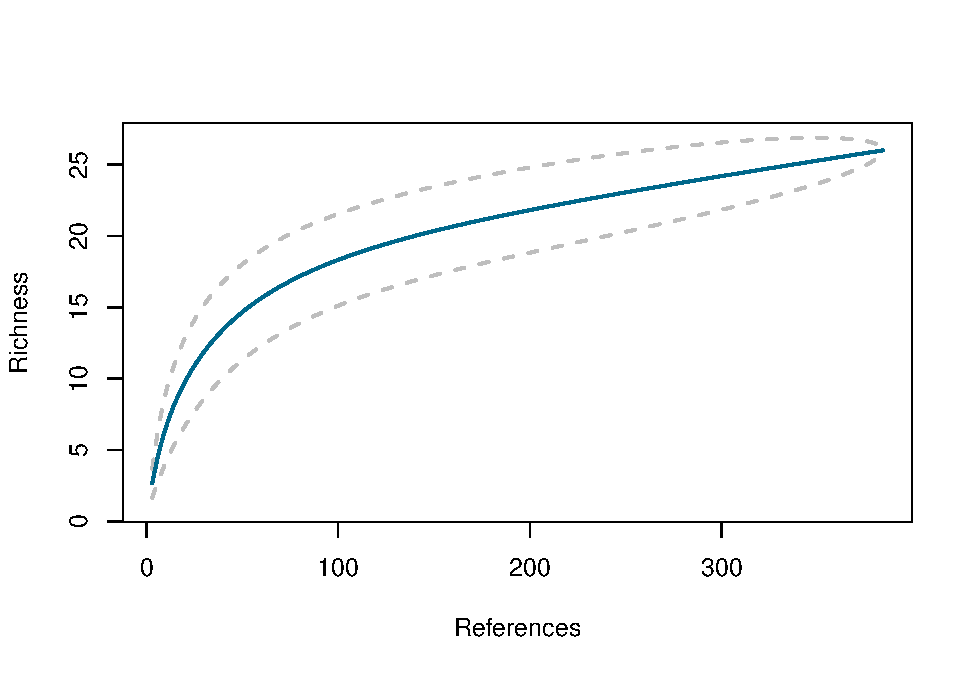
\includegraphics{MA_JJ_files/figure-latex/SACGenera-1.pdf}
	\caption{Sampling Accumulation Curve of fossil genera per reference}
\end{figure}

\FloatBarrier